\documentclass[crop,border=0pt]{standalone}

\usepackage{tikz}
\usetikzlibrary{positioning,scopes,shapes,arrows}

\begin{document}
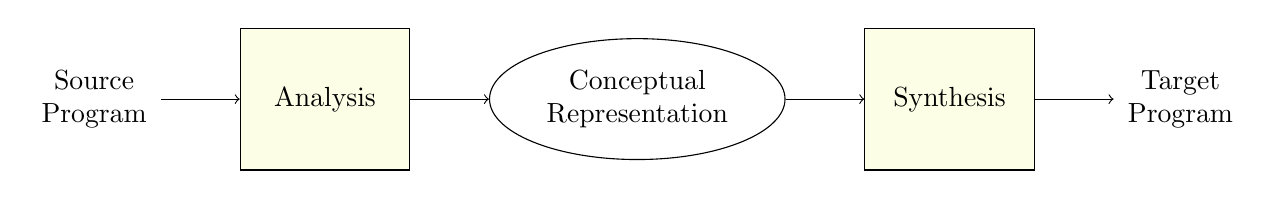
\begin{tikzpicture}[
  every node/.style={draw,rectangle,align=center,inner sep=5pt},
  module/.style={minimum height=1.8cm, text width=1.8cm, fill=green!10!yellow!10},
  repr/.style={ellipse,x radius=1.8cm, y radius=0.8cm}]

  \node [draw=none] (src) {Source\\Program};
  \node [module,right=of src] (analysis) {Analysis};
  \node [repr,right=of analysis] (repr) {Conceptual\\Representation};
  \node [module,right=of repr] (synthesis) {Synthesis};
  \node [draw=none,right=of synthesis] (tar) {Target\\Program};

  {[->]
    \draw (src) -- (analysis);
    \draw (analysis) -- (repr);
    \draw (repr) -- (synthesis);
    \draw (synthesis) -- (tar);
  }

\end{tikzpicture}
\end{document}
